\section{Experimental validation}\label{sec:experiments}

% Please add the following required packages to your document preamble:
% \usepackage{booktabs}
% \usepackage{graphicx}
\begin{table}[]
    \centering
    \caption{Hardware used in the experiments.}\label{tab:hardware}
    \resizebox{\columnwidth}{!}{%
    \begin{tabular}{@{}llrrrl@{}}
    \toprule
    \multicolumn{1}{c}{\textbf{}} &
      \multicolumn{1}{c}{\textbf{CPU}} &
      \multicolumn{1}{c}{\textbf{\begin{tabular}[c]{@{}c@{}}Freq\\ {[}\si{\giga\hertz}{]}\end{tabular}}} &
      \multicolumn{1}{c}{\textbf{\begin{tabular}[c]{@{}c@{}}Core\\ Count\end{tabular}}} &
      \multicolumn{1}{c}{\textbf{\begin{tabular}[c]{@{}c@{}}RAM\\ {[}\si{\giga\byte}{]}\end{tabular}}} &
      \multicolumn{1}{c}{\textbf{\begin{tabular}[c]{@{}c@{}}Operating\\ System\end{tabular}}} \\ \midrule
    \textbf{Cloudlet} &
      \begin{tabular}[c]{@{}l@{}}Intel\textregistered{} Core\texttrademark{}\\ i7-8700\end{tabular} &
      \num{3.2} &
      \num{6} &
      \num{32} &
      \begin{tabular}[c]{@{}l@{}}Ubuntu Server \\20.04 LTS \\Kernel v5.4.0\\\ \end{tabular} \\
    \textbf{Client} &
      \begin{tabular}[c]{@{}l@{}}Cortex-A72\\ (ARM v8)\end{tabular} &
      \num{2.0} &
      \num{4} &
      \num{8} &
      \begin{tabular}[c]{@{}l@{}}Ubuntu Server \\20.04 LTS \\Kernel v5.4.0\end{tabular} \\ \bottomrule
    \end{tabular}%
    }
\end{table}

In this section, we demonstrate the practical utility of \ac{CLEAVE} through a series of experiments on an emulated \ac{NCS} running between a client device and a cloudlet.
We aim to answer question relating to the ability of our framework to provide relevant, accurate, and repeatable measurements of the performance of \acp{NCS} deployed on edge computing infrastructure.

This section is structured in two parts.
\Cref{ssec:expsetup} details the experimental setup and describes the experiments performed.
\Cref{ssec:results} then presents and discusses the numerical results.

\subsection{Experimental Setup}\label{ssec:expsetup}

The \acl{NCS} employed for these experiments corresponds to an inverted pendulum, chosen for to its relative simplicity as well as prevalence in the field of automatic control as one of the fundamental examples of linear control.
The physical system (``plant''), represented in \cref{fig:invpend}, is implemented as a real-time discrete-time physical emulation using CLEAVE's API and a 2D physics library~\autocite{chipmunk2d,pymunk}, executed at a constant \SI{120}{\hertz}.
For the controller, a proportional-differential strategy is employed, implemented using the framework Controller API and the NumPy numeric computation library~\autocite{harris2020array}.
The plant and controller are then packaged into Docker\cite{merkel2014docker}, for ease of orchestration, deployment, and re-parametrization, as well as to mimic real-world deployment.

\begin{figure}
    \centering
    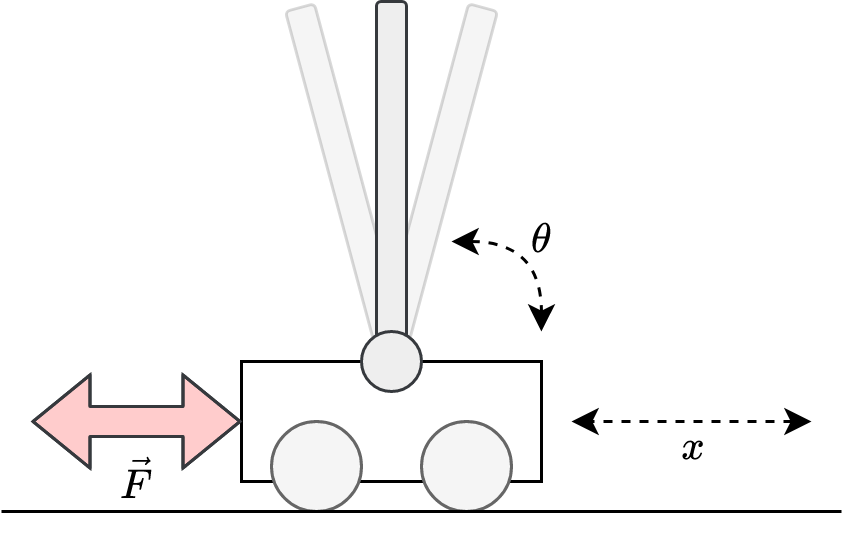
\includegraphics[width=.95\columnwidth]{images/inverted_pendulum.png}
    \caption{
        The two-dimensional inverted pendulum system.
        The cart moves on the X-axis, and the pendulum on top of it swings freely.
        The objective of the system is to balance the pendulum vertically through the application of horizontal forces on the cart.
    }\label{fig:invpend}
\end{figure}

We depict our experimental edge setup in \cref{fig:cleave:expsetup}.
It consists of \num{10} Raspberry Pi 4B  clients connected wirelessly to an IEEE 802.11n \ac{AP}; connected to the Ethernet backbone of this \ac{AP} is a general-purpose Cloudlet.
On top of this physical architecture we configure a Docker \emph{Swarm}~\cite{merkel2014docker,Swarm2021} managed centrally from the Cloudlet.
For each experimental scenario we deploy a number of control loops inside this Swarm, executing plant containers exclusively in the Raspberry Pi clients (up to a single plant per client) and controller containers in the Cloudlet.
Plants and controllers communicate using the \ac{UDP} over an overlay network which sits on top of and abstracts away the real network configuration.
Additionally, to obtain baseline results without the stochastic effects of the network, we employ a secondary ``local-only'' setup, in which plants and controllers are executed co-located on the Cloudlet.

\begin{figure}
    \centering
    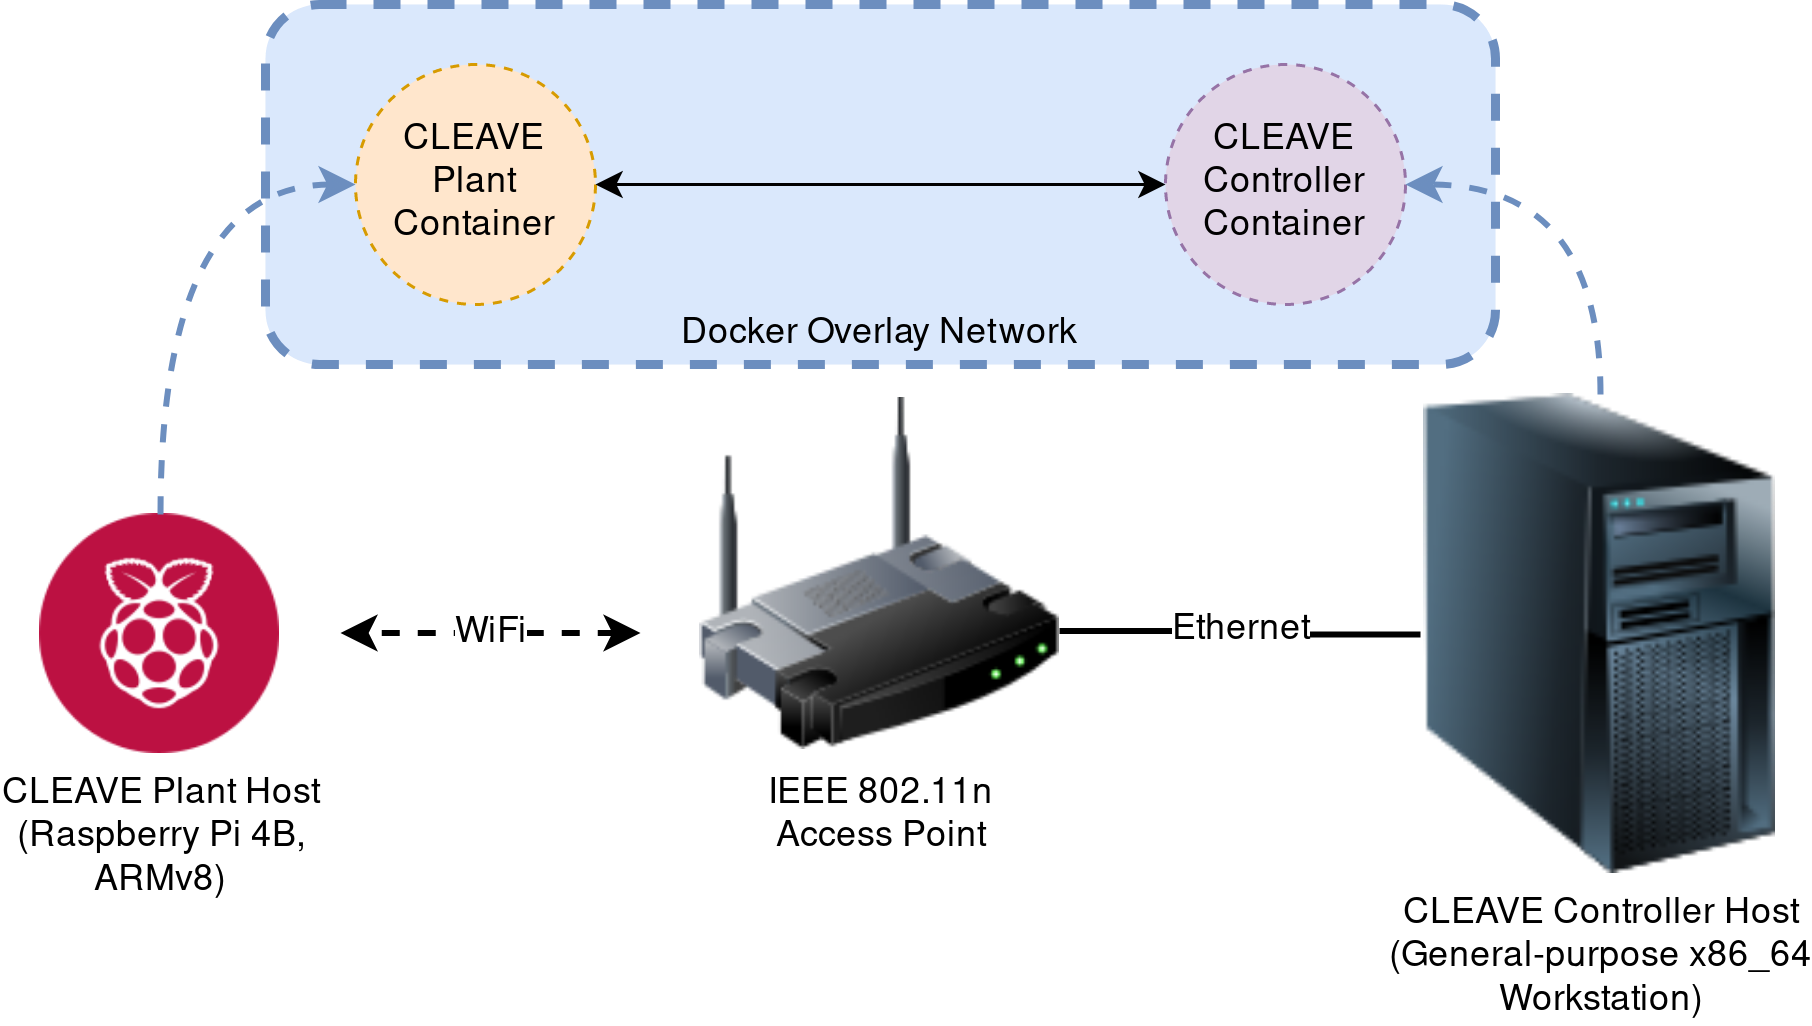
\includegraphics[width=.95\columnwidth]{images/CLEAVE_experiment_setup}
    \caption{Experimental setup. Containerized versions of the core CLEAVE emulation components are deployed inside a Docker Swarm Overlay Network spanning \num{10} Raspberry Pi 4B clients connected to a single Cloudlet over an IEEE 802.11n \ac{AP}.}\label{fig:cleave:expsetup}
    \todo[inline]{Change fig.}
\end{figure}

\subsubsection{Single Loop Baseline Scenarios}

We first run a series of single loop scenarios with varying parametrization of the controlled system.
\todo[inline]{Purpose of these scenarios?}
We modify:
\begin{itemize}
    \item the sampling rate of the Plant state, setting it to \SIlist[list-final-separator={, or }]{5;10;20;40;60}{\hertz};
    \item the responsiveness of the Controller, by adding fixed delays of  \SIlist[list-final-separator={, or }]{0;25;50;100}{\milli\second} after the processing of each sample.
\end{itemize}
We repeat each combination of these parameters at least \num{10} times, for both the networked and ``local-only'' setups; experiments with interesting and relevant results are then repeated an additional \num{20} times for better statistical significance in the results.
Each repetition lasts for \SI{5}{\minute}, during which we collect detailed data on both the state of the controlled system as well as on the data sent over the network.

\subsubsection{Realistic Scenario with Resource Contention}

Next, we run a more complex scenario to validate the utility of \ac{CLEAVE} in a more realistic setting where network resources are shared with video stream traffic.
Video analytics is one of the main proposed use cases for edge computing~\cite{Ananthanarayanan2017Analytics,Yi2017Analytics,Wang2018Analytics}, and thus we foresee edge \ac{NCS} deployments being deployed in parallel with such applications in the future.

In this scenario, we deploy \num{6} control loops on the experimental setup depicted in \cref{fig:cleave:expsetup}.
On the remaining \num{4} clients we run the \emph{iperf3}~\cite{iperf3} traffic load generator, each generating \SI[per-mode=symbol]{6.5}{\mega\bit\per\second} of \ac{UDP} uplink traffic.
This traffic emulates the load generated on the network by \SI{1080}{p} Full-HD video streaming, originating from the clients and terminating in the cloudlet.
We execute this scenario with \ac{NCS} plant sampling rates of \SIlist{20;40;60}{\hertz}.
Each sampling rate configuration is run for \SI{5}{\minute}, and then repeated \num{30} times to obtain statistical significance.

\subsection{Results}\label{ssec:results}

The results presented below provide valuable insights on both system limits and on the chosen \ac{NCS} itself, as well as on the capabilities of \ac{CLEAVE}.

\subsubsection{Single Plant Scenario}

We begin with a simple analysis of the stability of the Plant, as \ac{CLEAVE} allows for straightforward and repeatable analysis of relevant metrics.  
For instance, \cref{fig:topple:fraction} shows a visualization of the fraction of plants that toppled in each scenario.
These Plants were identified simply by analyzing the emulation data --- instances whose pendulum angles reached values above a certain value\footnote{This value will depend on the parametrization of the controller, and in this case corresponds to \SI{20}{\degree}, or \SI{0.35}{\radian}.} were marked as ``toppled''.

\begin{figure}
    \centering
    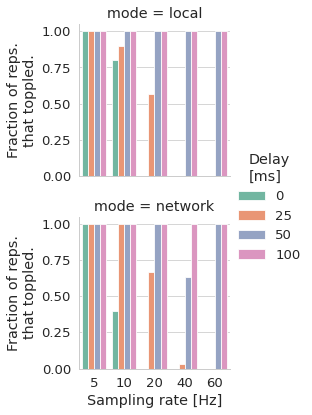
\includegraphics[width=.8\columnwidth]{topple_fraction.png}
    \caption{Fraction of plants that toppled, per experimental setup.}%
    \label{fig:topple:fraction}
\end{figure}

\Ac{CLEAVE} also allows for more fine-grained analysis of stability.
\Cref{fig:topple:rms} shows the \ac{RMS} of the angles for each setup, averaged over all repetitions of each experiment.
This figure shows an intuitive but important result --- less stable setups show higher amplitude in the oscillations of their penduli.

\begin{figure}
    \centering
    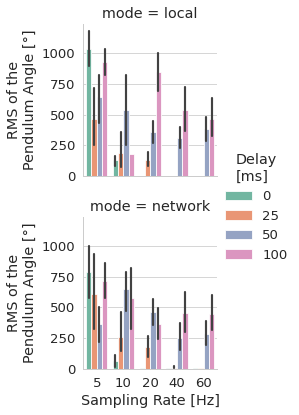
\includegraphics[width=.8\columnwidth]{angle_rms.png}
    \caption{\Ac{RMS} of the pendulum angles averaged over all runs for each scenario.
    Error bars indicate \SI{95}{\percent} \acp{CI}.}%
    \label{fig:topple:rms}
\end{figure}

Finally, we showcase \ac{CLEAVE}'s ability to obtain network performance data from the experiments.
\Cref{fig:network} shows average \acp{RTT}s and packet losses per scenario.

\begin{figure}
    \centering
    % 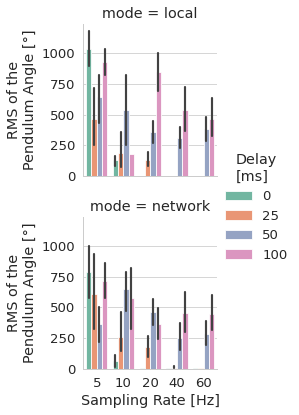
\includegraphics[width=.8\columnwidth]{angle_rms.png}
    \caption[caption]{Mean \acp{RTT} and packet losses for each scenario; \acp{RTT} were calculated by subtracting the synthetic delay from the absolute end-to-end latency\textsuperscript{a}. Error bars indicate \SI{95}{\percent} \acp{CI}.}%
    \small\textsuperscript{a} The systematic offset of \SI{2}{\milli\second} on scenarios with synthetic delay is an artifact of our implementation, and will be fixed in the next release of the framework.
    \label{fig:network}
\end{figure}


\todo[inline]{Discuss which network results to add.}

\subsubsection{Realistic Scenario}

\begin{figure}
    \centering
    \begin{subfigure}[h]{\columnwidth}
        \centering
        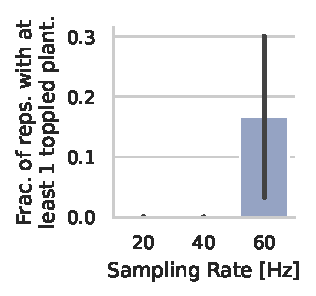
\includegraphics[width=.8\columnwidth]{video_topple_frac}
        \caption{}\label{fig:video:toppled}
    \end{subfigure}\\%
    \begin{subfigure}[h]{\columnwidth}
        \centering
        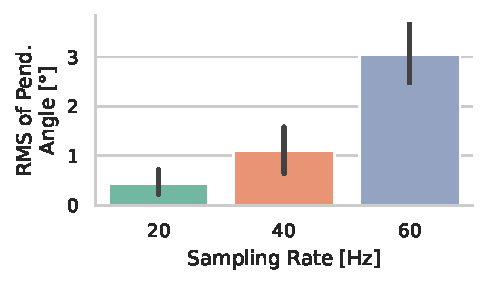
\includegraphics[width=.8\columnwidth]{video_angle_rms}
        \caption{}\label{fig:video:rms}
    \end{subfigure}%
    \caption{
        Stability metrics for the realistic scenario.
        \labelcref{fig:video:toppled} shows the fraction of repetitions of each scenario in which \emph{at least} one plant failed to maintain stability and toppled.
        \labelcref{fig:video:rms} shows the \ac{RMS} for the pendulum angles for each scenario, only considering data from plants that did not topple.
        Error bars indicate \SI{95}{\percent} \ac{CI} in both plots.
    }\label{fig:video:stability}
\end{figure}

\begin{figure}
    \centering
    \begin{subfigure}[h]{\columnwidth}
        \centering
        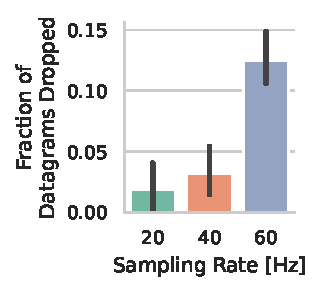
\includegraphics[width=.8\columnwidth]{video_drop_frac}
        \caption{}\label{fig:video:drop}
    \end{subfigure}\\%
    \begin{subfigure}[h]{\columnwidth}
        \centering
        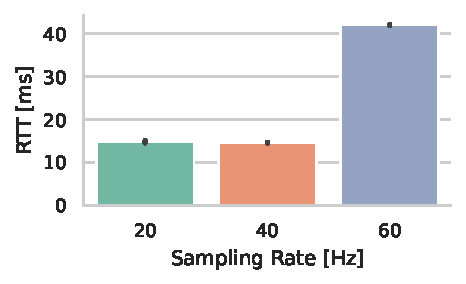
\includegraphics[width=.8\columnwidth]{video_rtt}
        \caption{}\label{fig:video:rtt}
    \end{subfigure}%
    \caption{
        Network metrics for the realistic scenario.
        \labelcref{fig:video:drop} shows the fraction of \ac{UDP} datagrams dropped, averaged over all plants and repetitions per scenario.
        \labelcref{fig:video:rtt} shows the measured end-to-end plant-side \ac{RTT}, averaged over all plants and repetitions per scenario.
        Error bars indicate \SI{95}{\percent} \ac{CI} in both plots.
    }\label{fig:video:network}
\end{figure}